\documentclass[border=1mm]{standalone}

% ---- Packages ---- %
\usepackage[utf8]{inputenc}
\usepackage[ngerman]{babel}
\usepackage{tikz}
\usetikzlibrary{arrows.meta}
\usetikzlibrary{calc}
\usetikzlibrary{shapes}
\usetikzlibrary{positioning,arrows}

\definecolor{rwth-blue}{HTML}{00549F}
\definecolor{rwth-lblue}{HTML}{8EBAE5}
\definecolor{rwth-llblue}{HTML}{C7DDF2}

\begin{document}	

	\begin{tikzpicture}[fill=rwth-blue,ultra thick]
		
		\tikzstyle{myarrows}=[line width=1mm,draw=rwth-blue,-triangle 45,postaction={draw, line width=3mm, shorten >=4mm, -}]
		
		\clip (0,0) rectangle (14,-15);
			
		%\draw[help lines] (0,0) grid (14,-15);
			
		\node[above,align=center] (Text1) at (3,-3) { 1) \textbf{Steckmodule} ermöglichen \\ einen leichten Transport \\ und Aufbau };
		\node[below] (Bild1) at (3,-3) {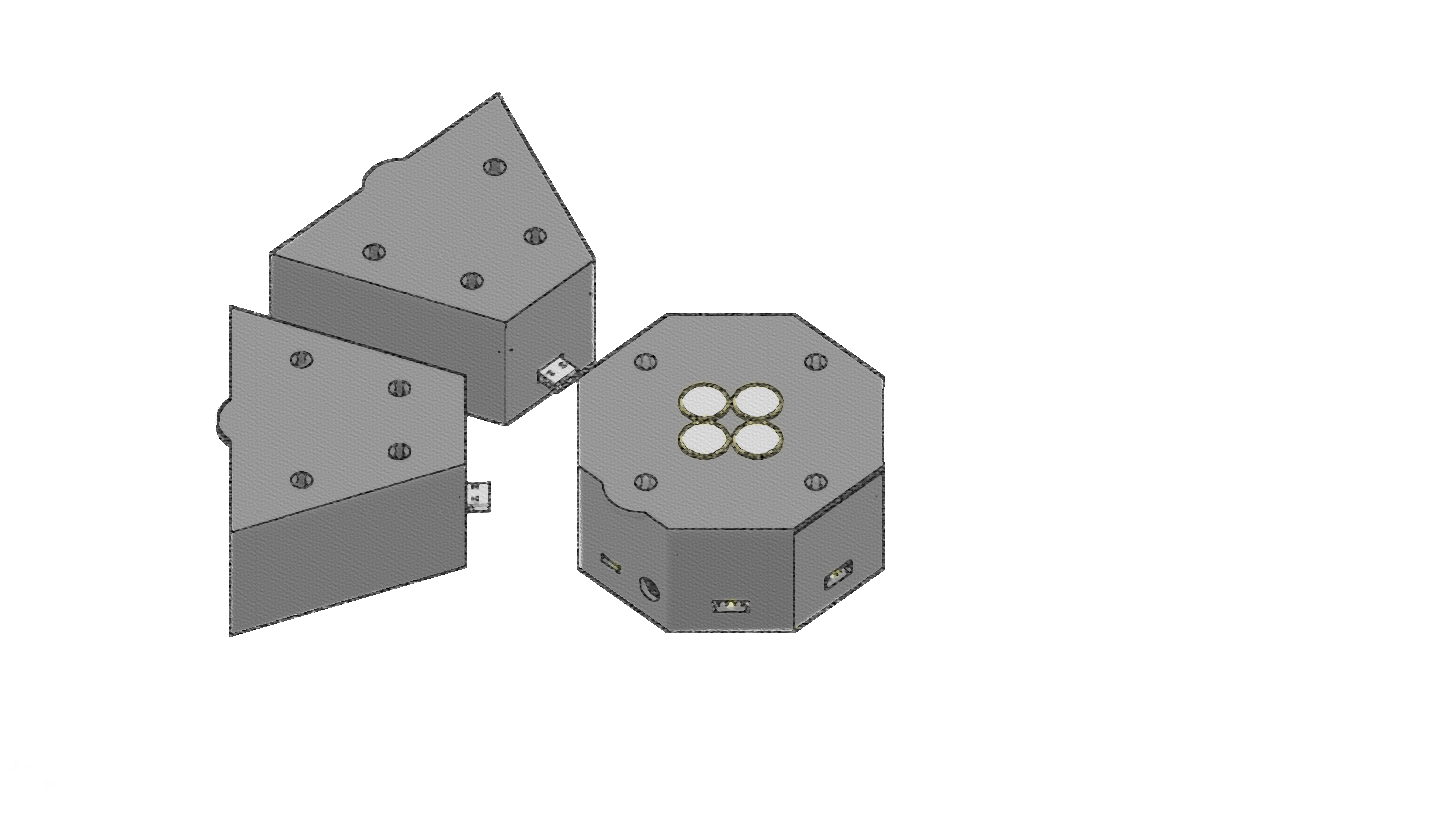
\includegraphics[scale=0.25]{../../CAD_Bilder/Flyer_Bilder/IMG_1344.png}};
			
		\node[above,align=center] (Text2) at (11,-2.5) { 2) \textbf{Erkennen} einer \\ Handgeste durch \\ Detektion von \\ Lichtreflektionen };
		\node[below] (Bild2) at (11,-2.5) {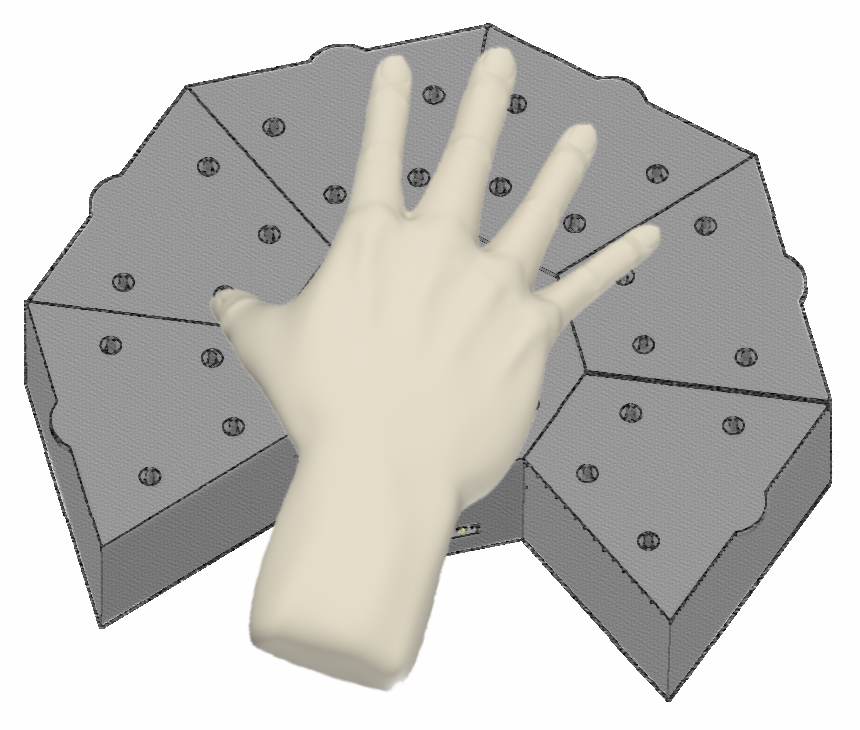
\includegraphics[scale=0.25]{../../CAD_Bilder/Flyer_Bilder/IMG_1342.png}};
			
		\node[above,align=center] (Text3) at (10,-10) { 3) Interpretation der \\ Reflexionsmuster \\ mit Hilfe eines \\ \textbf{Machine Learning} \\ Algorithmus };
		\node[below] (Bild3) at (10,-10) {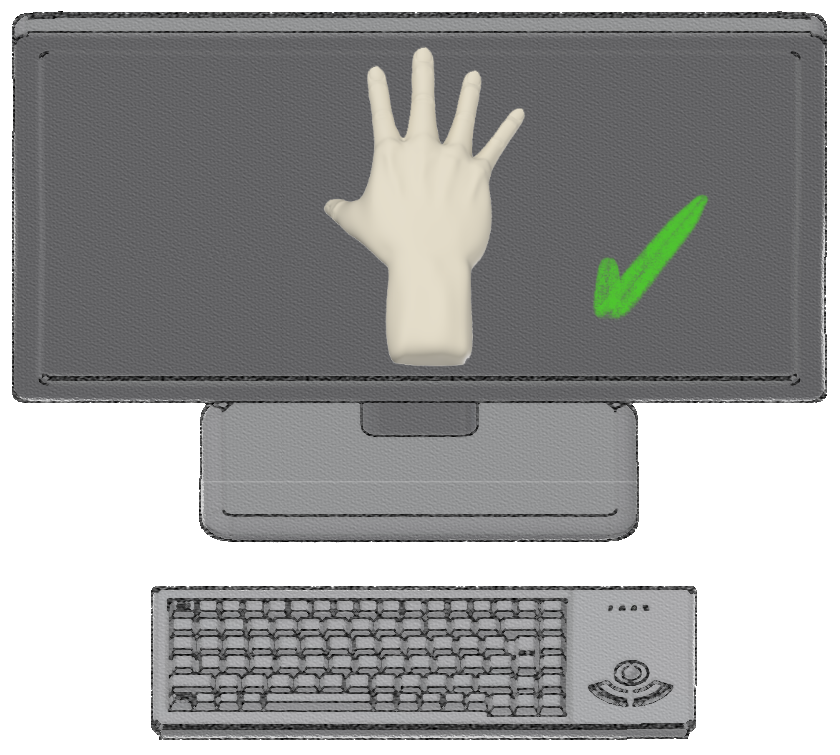
\includegraphics[scale=0.25]{../../CAD_Bilder/Flyer_Bilder/IMG_1340.png}};
			
		\node[above,align=center] (Text4) at (3,-10) { 4) \textbf{Steuern} eines Endgeräts };
		\node[below] (Bild4) at (3,-10) {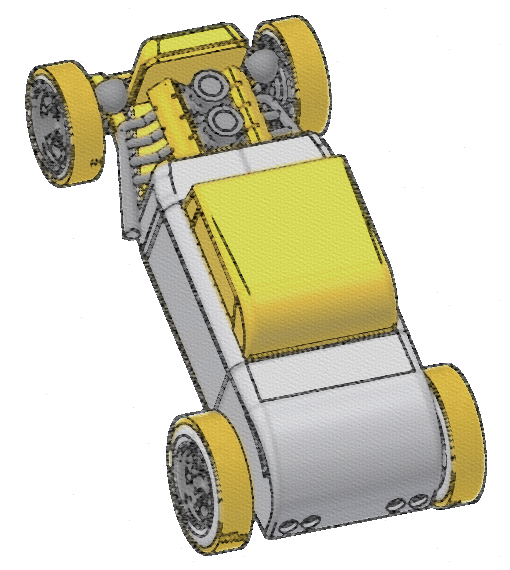
\includegraphics[scale=0.25]{../../CAD_Bilder/Flyer_Bilder/IMG_1341.png}};
			
		\path[myarrows]
    		(Bild1) edge[bend left] node {} (Bild2);
    			
    	\path[myarrows]
    		(Bild2) edge[bend left] node {} (Bild3);
			
		\path[myarrows]
    		(Bild3) edge[bend left] node {} (Bild4);
			
	\end{tikzpicture}
		
\end{document}